%%%%%%%%%%%%%%%%%%%%%%%%%%%%%%%%%%%%%%%%%
% kaobook
% LaTeX Template
% Version 1.2 (4/1/2020)
%
% Authors:
% Federico Marotta (federicomarotta@mail.com)
% Based on the doctoral thesis of Ken Arroyo Ohori (https://3d.bk.tudelft.nl/ken/en)
% and on the Tufte-LaTeX class.
% Modified for LaTeX Templates by Vel (vel@latextemplates.com)
%
% License:
% CC0 1.0 Universal (see included MANIFEST.md file)
%
%%%%%%%%%%%%%%%%%%%%%%%%%%%%%%%%%%%%%%%%%

%----------------------------------------------------------------------------------------
%	PACKAGES AND OTHER DOCUMENT CONFIGURATIONS
%----------------------------------------------------------------------------------------

\documentclass[
	fontsize=10pt, % Base font size
	twoside=false, % Use different layouts for even and odd pages (in particular, if twoside=true, the margin column will be always on the outside)
	open=any, % If twoside=true, uncomment this to force new chapters to start on any page, not only on right (odd) pages
	%chapterprefix=true, % Uncomment to use the word "Chapter" before chapter numbers everywhere they appear
	%chapterentrydots=true, % Uncomment to output dots from the chapter name to the page number in the table of contents
	numbers=noenddot, % Comment to output dots after chapter numbers; the most common values for this option are: enddot, noenddot and auto (see the KOMAScript documentation for an in-depth explanation)
	%draft=true, % If uncommented, rulers will be added in the header and footer
	%overfullrule=true, % If uncommented, overly long lines will be marked by a black box; useful for correcting spacing problems
]{kaobook}

% Set the language
\usepackage[english]{babel} % Load characters and hyphenation
\usepackage[english=british]{csquotes} % English quotes

% Load packages for testing
%\usepackage{blindtext}
%\usepackage{showframe} % Uncomment to show boxes around the text area, margin, header and footer
%\usepackage{showlabels} % Uncomment to output the content of \label commands to the document where they are used

% Load the bibliography package
\usepackage{styles/kaobiblio}
\addbibresource{main.bib} % Bibliography file

% Load mathematical packages for theorems and related environments. NOTE: choose only one between 'mdftheorems' and 'plaintheorems'.
\usepackage{styles/mdftheorems}
%\usepackage{styles/plaintheorems}

\graphicspath{{examples/documentation/images/}{images/}} % Paths in which to look for images

\makeindex[columns=3, title=Alphabetical Index, intoc] % Make LaTeX produce the files required to compile the index

\makeglossaries % Make LaTeX produce the files required to compile the glossary

\makenomenclature % Make LaTeX produce the files required to compile the nomenclature

% Reset sidenote counter at chapters
%\counterwithin*{sidenote}{chapter}

%----------------------------------------------------------------------------------------

\begin{document}

%----------------------------------------------------------------------------------------
%	BOOK INFORMATION
%----------------------------------------------------------------------------------------

%\titlehead{The \texttt{kaobook} class}
\subject{Diploma Thesis}

\title{Class-E Tesla Coil}
%\subtitle{Customise this page according to your needs}

\author{Marcher Simon\\Peyer Kassandra\\Felix Hamrle}

\date{\today}

%\publishers{An Awesome Publisher}

%----------------------------------------------------------------------------------------

\frontmatter % Denotes the start of the pre-document content, uses roman numerals

%----------------------------------------------------------------------------------------
%	OPENING PAGE
%----------------------------------------------------------------------------------------

%\makeatletter
%\extratitle{
%	% In the title page, the title is vspaced by 9.5\baselineskip
%	\vspace*{9\baselineskip}
%	\vspace*{\parskip}
%	\begin{center}
%		% In the title page, \huge is set after the komafont for title
%		\usekomafont{title}\huge\@title
%	\end{center}
%}
%\makeatother

%----------------------------------------------------------------------------------------
%	COPYRIGHT PAGE
%----------------------------------------------------------------------------------------

\makeatletter
\uppertitleback{\@titlehead} % Header

\lowertitleback{
	\textbf{Disclaimer}\\
	You can edit this page to suit your needs. For instance, here we have a no copyright statement, a colophon and some other information. This page is based on the corresponding page of Ken Arroyo Ohori's thesis, with minimal changes.
	
	\medskip
	
	\textbf{No copyright}\\
	\cczero\ This book is released into the public domain using the CC0 code. To the extent possible under law, I waive all copyright and related or neighbouring rights to this work.
	
	To view a copy of the CC0 code, visit: \\\url{http://creativecommons.org/publicdomain/zero/1.0/}
	
	\medskip
	
	\textbf{Colophon} \\
	This document was typeset with the help of \href{https://sourceforge.net/projects/koma-script/}{\KOMAScript} and \href{https://www.latex-project.org/}{\LaTeX} using the \href{https://github.com/fmarotta/kaobook/}{kaobook} class.
	
	The source code of this book is available at:\\\url{https://github.com/fmarotta/kaobook}
	
	(You are welcome to contribute!)
	
	\medskip
	
	\textbf{Publisher} \\
	First printed in May 2019 by \@publishers
}
\makeatother

%----------------------------------------------------------------------------------------
%	DEDICATION
%----------------------------------------------------------------------------------------

%\dedication{
%	The harmony of the world is made manifest in Form and Number, and the heart and soul and all the poetry %of Natural Philosophy are embodied in the concept of mathematical beauty.\\
%	\flushright -- D'Arcy Wentworth Thompson
%}

%----------------------------------------------------------------------------------------
%	OUTPUT TITLE PAGE AND PREVIOUS
%----------------------------------------------------------------------------------------

% Note that \maketitle outputs the pages before here

% If twoside=false, \uppertitleback and \lowertitleback are not printed
% To overcome this issue, we set twoside=semi just before printing the title pages, and set it back to false just after the title pages
\KOMAoptions{twoside=semi}
\maketitle
\KOMAoptions{twoside=false}

%----------------------------------------------------------------------------------------
%	PREFACE
%----------------------------------------------------------------------------------------

%\input{chapters/preface.tex}

%----------------------------------------------------------------------------------------
%	TABLE OF CONTENTS & LIST OF FIGURES/TABLES
%----------------------------------------------------------------------------------------

\begingroup % Local scope for the following commands

% Define the style for the TOC, LOF, and LOT
%\setstretch{1} % Uncomment to modify line spacing in the ToC
%\hypersetup{linkcolor=blue} % Uncomment to set the colour of links in the ToC
\setlength{\textheight}{23cm} % Manually adjust the height of the ToC pages

% Turn on compatibility mode for the etoc package
\etocstandarddisplaystyle % "toc display" as if etoc was not loaded
\etocstandardlines % toc lines as if etoc was not loaded

\tableofcontents % Output the table of contents

\listoffigures % Output the list of figures

% Comment both of the following lines to have the LOF and the LOT on different pages
\let\cleardoublepage\bigskip
\let\clearpage\bigskip

\listoftables % Output the list of tables

\endgroup

%----------------------------------------------------------------------------------------
%	MAIN BODY
%----------------------------------------------------------------------------------------

\mainmatter % Denotes the start of the main document content, resets page numbering and uses arabic numbers
\setchapterstyle{kao} % Choose the default chapter heading style

\pagelayout{wide} % No margins
\addpart{The Tesla Coil}
\pagelayout{margin} % Restore margins
\setchapterstyle{kao}
\setchapterpreamble[u]{\margintoc}

\chapter{Theory of Operation} % How it should work in theory
\labch{tc-theory-of-operation}

The tesla coil was invented by Nikola Tesla in 1891. His vision was to use this technology to wirelessly transmit power to people all over the world. While his plans didn't meet the expectations by far, he still opened up a whole new field of physics, which today helps power the modern world.

Tesla coils come in a huge variety of sizes, power and modes of operation. From simple spark gap tesla coils, which consist of only a few passive components, to solid state tesla coils, whose only limitations are one's technical skills, every single one amazes anew by combining the world of High Voltage and High Frequency.

In order to understand the class E topology which this thesis is about, we have to understand the basics first. 

\section{The Tesla Resonator}

A tesla resonator, also called tesla coil, is a resonant transformer consisting of two loosely coupled air-cored windings: the primary and secondary coil. The primary coil, hooked up to the driver circuit on one side and grounded on the other, is usually made out of every few turns of thick wire. It is placed around the bottom of the secondary coil, either shaped like an flat spiral, a concentric cylinder, or at any angle in between. The secondary coil on the other hand has a lot more turns and is a lot higher.

\begin{marginfigure}[*-5]
\includegraphics[width=\textwidth]{simon/images/teslaCoilStrayCapacitance.png}
\caption{Stray capacitances of the secondary coil}
\labfig{teslaCoilStrayCapacintance}
\end{marginfigure}

As every real component, a coil has parasitic effects. The one relevant to a tesla coil's operation is the parasitic capacitance. A capacitance is just two different isolated voltage potentials, which is exactly, what we have along every single winding of a coil. This makes clear that every coil is actually an LC oscillator. The lower the inductance and capacitance of the coil, the higher the resonant frequency. This means that in order to lower the frequency to the desired one, many tesla coils have a top load, which, amongst others, acts like as an additional capacity towards ground.

If a high voltage, whose frequency is the resonant frequency of the secondary, is now applied to the primary coil, the LC circuit in the secondary coil starts oscillating and a very high voltage builds up gradually. Depending on the size and power of the tesla coil, this voltage can range from a few thousand to a few million volts. Once the voltage is high enough to ionise the air around the top\sidenote{This usually happens at a designated spark point}, it quickly discharges and the cycle starts over again.

\section{Exciting The Resonator}

There are various circuits which can be used for the excitation of the coil. Depending on the desired spark length, size\sidenote{The size of the secondary coil mostly determines its resonant frequency}, sensitivity to external effects, noise level and efficiency, different tesla coil drivers can be used. While Tesla's coils all used a spark gap topology, today we are able to use solid state devices to control the coil instead.

\subsection{The Spark Gap Tesla Coil}

\begin{marginfigure}
\includegraphics[width=\textwidth]{simon/images/sparkGapTeslaCoil.png}
\caption{A simple spark gap tesla coil}
\labfig{teslaCoilStrayCapacintance}
\end{marginfigure}

The simplest of all drivers is the spark gap driver. In the first stage, the 230V mains voltage is transformed to a few kilovolts. Neon sign or microwave transformers are popular choices for this task. The capacitor gets charged up until the voltage is high enough to break through the spark gap. The spark gap then has a very low resistance and allows the current to oscillate between the capacitor and the primary coil. This oscillation frequency is usually in the order of ten to hundred kilohertz and is the same frequency as the resonant frequency of the secondary coil. In every cycle, a little energy is transferred to the secondary via the magnetic coupling of the coils. When the voltage in the secondary gets too high, a breakout occurs. This can happen one or more times within a period of the AC mains voltage. Once all the energy in the primary circuit has been transferred to the secondary or dissipated as heat, the spark gap \enquote{quenches} allowing the capacitor to charge up again.

Today, spark gap tesla coils are mostly only used for educational purposes anymore. Due to their many \textbf{disadvantages} they are avoided when power efficiency and noise level play a role. The disadvantages most worth mentioning include:

\begin{itemize}
\item A spark gap dissipates a lot of power, part of it in heat and part of in in creating a lot of ozone, which also posses a health hazard, when operated in closed rooms.
\item The rapid igniting and quenching of the spark gap creates a lot of noise.
\item The whole operation cycle only depends on passive component values, which makes it impossible to control the power output and play music.
\end{itemize}

\subsection{Solid State Tesla Coils}

Aside from vacuum tube tesla coils, which have existed before, semiconductor technology\sidenote{Unlike relays or hard disk drives, their semiconductor counterparts have no moving components. Hence the name \enquote{solid state}.} opened up a whole new world of possibilities for tesla coils. It was now possible to build up sophisticated amplifier circuits to excite the primary coil. Some of them still rely on resonant circuits, others use feedback loops to self-excite the primary coil, and again others use ICs to control the driver.

The most common solid state topologies include:
\begin{itemize}
\item Slayer exciter
\item Half-bridge / full-bridge (single or dual resonant)
\item Class E
\end{itemize}

\subsubsection{Slayer Exciter Circuit}

The slayer exciter topology is the most common under hobbyist coilers\sidenote{This is what people building tesla coils often call themselves}, because it's by far the simplest one, only consisting of very few components. At it's hard sits the Transistor T controlling the current through the primary coil L1. When first powering on the circuit, current flows through R into the base of T, allowing current to flow through L1, creating a magnetic field.\sidenote{It is important that the winding directions of the two coils are opposing each other, so that the voltage across the secondary won't be inverted.}\todo{Why is the winding direction the way it is?} The rapid change in the field induces a high voltage in the secondary coil L2. The parasitic capacitance C of L2 however only lets the voltage across it rise slowly, therefore pushing the potential of the bottom of the lower end of L2 to a negative voltage. As soon as the voltage falls below -0.7V, the diode D starts conducting and limits the negative voltage while providing current to charge up C\sidenote{The diode could be left out, since the base emitter junction also acts as diode, but in the most cases this damages the transistor}. Additionally, since the base emitter voltage is now negative, T stops conducting. This causes the magnetic field to start collapsing, causing the potential at the base to slowly rise, until T starts conducting again. The circuit is now in it's initial state, except that C is now charged to a high voltage and the process starts over again.

Since the timing of the circuit only depends on the values of L1, L2, and C, the circuit tunes itself, which makes it very stable to operate. But because of its simplicity it comes with a few disadvantages. Firstly, when T is conducting, it basically shorts L1, which leads to a high current and therefore power dissipated in T. This power can be reduced by choosing R to be rather high. This reduces the base current and therefore also the collector current. While this helps reducing the power dissipation it also reduces the output power of the coil. With a bit of extra complexity this circuit can however be made more efficient\todo{add some source}.

\begin{figure}[h!]
\centering
\begin{circuitikz}[european, american inductors]
  \draw (2,4) to[short, *-] (0,4) to[battery, l=V] (0,0) node[ground]{};
  \draw (2,4) to[R, l=R] (2,1) to[D-, l=D] (2,0) node[ground]{};
  \draw (4,1.5) node[npn](npn){T};
  \draw (2,4) -- (4,4) to[L, l_=L\textsubscript{1}] (npn.C);
  \draw (npn.C) ++(-.2,.4) node[circ]{};
  \draw (npn.E) -- (4,0) node[ground]{};
  \draw (npn.B) to[short, -*] (2,1.5);
  \ctikzset{inductors/coils=10, inductors/width=2}
  \draw (5,.5) to[L, l=L\textsubscript{2}] (5,4) -- (6,4) to[C, l=C] (6,0) node[ground]{};
  \draw (5,4) ++(.2,-.4) node[circ]{};
  \draw (3,1.5) to[short, *-] (3,.5) to[crossing] (5,.5);
\end{circuitikz}
\caption{Slayer exciter circuit}
\end{figure}

\subsubsection{Half-Bridge / Full-Bridge}

This design drives the primary coil by a half or full bridge. While this requires large and expensive power MOSFETs or IGBTs as well as carefully designed GDTs\sidenote{Gate drive transformer}, it offers a lot of flexibility and power up to many kW.

\begin{figure}
\captionsetup[subfigure]{labelformat=empty}
\centering
\begin{subfigure}{.5\textwidth}
  \centering
  \begin{circuitikz}[european, american inductors]
  \draw (0,0) node[nigfete](n2){};
  \draw (n2.S) node[tlground](g1){};
  \draw (0,2) node[nigfete](n1){};
  \draw (n1.S) -- (n2.D);
  \draw (0,1) node[circ]{} to[L] (2,1) node[circ]{};
  \draw (g1 -| 2,2) node[tlground]{} to[C] (2,1) to[C] (n1.D -| 2,1) -- ++(-2,0);
  \draw (n1.D -| 1,2) node[vcc]{};
  \end{circuitikz}
  \caption{Half bridge design}
\end{subfigure}%
\begin{subfigure}{.5\textwidth}
  \centering
  \begin{circuitikz}[european, american inductors]
  \draw (0,0) node[nigfete](n2){};
  \draw (n2.S) node[tlground](g1){};
  \draw (0,2) node[nigfete](n1){};
  \draw (n1.S) -- (n2.D);
  \draw (0,1) node[circ]{} to[L] (2,1) node[circ]{};
  \draw (2,0) node[nigfete, xscale=-1](n4){};
  \draw (2,2) node[nigfete, xscale=-1](n3){};
  \draw (n3.S) -- (n4.D);
  \draw (n4.S) node[tlground]{};
  \draw (n1.D -| 1,2) node[vcc]{};
  \draw (n3.D) -- (n1.D);
  \end{circuitikz}
  \caption{Full bridge design}
\end{subfigure}
\end{figure}

The decision between a half bridge or full bridge design is a tradeoff between the number of parts and the output power. Due to the two capacitors in the half bridge design, the second end of the primary coil is biased at  \(\nicefrac{V_{CC}}{2}\), which means that the maximum voltage across the primary coil can also be only \(\nicefrac{V_{CC}}{2}\). However, a working half bridge design can rather easily be expanded to a full bridge design, which can then utilize the whole supply voltage.

A half or full bridge design can be deployed either single or dual resonant\sidenote{Mostly known as Dual Resonant SSTC or DRSSTC}. In order to turn a single resonant design into a double resonant design, a capacitor is added to the primary circuit which turns it into an resonator with the same resonant frequency as the secondary coil. Since the reactance of an LC circuit is the lowest at its resonant frequency, it draws a lot more current than the primary coil alone, resulting in more power transmitted to the secondary coil.

This design is often used for medium-sized to large tesla coils due to its high output power. However, due to the MOSFETs\sidenote{Or other switching device, like an IGBT} switching a high current at a high voltage, a lot of power is dissipated and they have to be adequately cooled. The stress on the MOSFETs can be reduced a bit by interrupting\sidenote{Turning the coil off and on very quickly} the tesla coil. Additionally, this allows the plasma channels to quench during each interrupting cycle, raising its resistance and therefore the breakout voltage, which in turn raises the length of the arcs. So this technique lowers the stress on the switching devices, lowers the input power and raises the arc length. The only drawback is that the arcs sound a lot harsher and louder.

A big advantage of the bridge design is, that unless a dual resonant design is chosen, the switching frequency is only determined by the circuit driving the bridge. This allows it to work across a very wide range of frequencies and even follow the slightly changing resonant frequency of the secondary coil in real time.

\subsubsection{Class E}

This topology uses a class E RF amplifier to produce the necessary power for driving the primary coil. By utilizing a technique called ZVS\sidenote{Zero voltage switching} and ZCS\sidenote{Zero current switching}, the dissipated power in the switching device is drastically reduced, making this type of amplifier nearly 100\% efficient in theory. A class E amplifier is capable of switching very high frequencies, which makes it an ideal driver for smaller tesla coils operating at a few MHz.

\section{Class E Amplifier}
The class E amplifier was first introduced by N. O. Sokal and A. D. Sokal in 1975. Since then there have been many attempts to derive  and then simplify analytical design equations.

\subsection{Theory of Operation}

\subsection{The Class-E Amplifier as Tesla Coil Driver}

\section{Playing Music}

\setchapterstyle{kao}
\setchapterpreamble[u]{\margintoc}

\chapter{Design and Simulation} % How I thought it was going to work
\labch{tc-design-and-simulation}

\textbf{Disclaimer:} This process was a lot more length and tedious than depicted in the following chapter. It mostly consisted of trial and error, which started with an more or less educated guess and ended in cluelessness and despair. But those errors don't add a lot of value to understanding the topic, so I won't go into much detail.

\section{The Coils}

The goal was to design an air coil with a resonant frequency of 4MHz. This frequency was chosen, since it is high enough to work well with an class E amplifier, but low enough to not run into too many RF related problems. It was also already known to have worked with a few other class E tesla coils.

\subsection{Rough Estimation of the Secondary Coil}

The inductance of a single-layered air solenoid coil can be calculated with

\begin{equation}\label{eq-inductivity}
    L = \mu_0 \frac{N^2 A}{l}
\end{equation}

The parasitic capacitance, depending on its length \(l\) and its diameter \(D\) can be calculated with\sidecite{self-capacitance}

\begin{equation}\label{eq-parasitic-capacitance}
    C_L = \frac{4\varepsilon_0}{\pi} \cdot l \cdot \left( 1 + 0.8249 \frac{D}{l} + 2.329 \left(\frac{D}{l}\right)^{1.5}\right)
\end{equation}

Defining the length to diameter ratio of the coil to be 4, and \(d_w\) to be the diameter of the wire, both formulas can be rewritten to only depend on \(l\) and \(d_w\). 

\begin{equation}
    L = \mu_0 \frac{l^3\ \pi}{32 d_w^2}
\end{equation}

\begin{equation}
    C_L = \frac{4\varepsilon_0}{\pi} \cdot l \cdot 1.49735
\end{equation}

Those equations can then be set into the formula for the resonant frequency of an LC circuit.

\begin{equation}
    f = \frac{1}{2\pi \cdot \sqrt{0.1872 \cdot \dfrac{1}{d_w^2} \cdot \mu_0 \varepsilon_0 \cdot l^4}}
\end{equation}

Rearranging the equation to \(l\)

\begin{equation}
    l = \frac{1}{\sqrt[\scalebox{1}{4}]{4\pi^2 f^2 \cdot0.1872 \cdot \dfrac{1}{d_w^2} \cdot \mu_0 \varepsilon_0}}
\end{equation}

With a frequency of 4MHz and a wire diameter of 0.35mm, the length of the coil turns out to be around 100mm and the diameter therefore around 25mm.

Due to the materials available, a 30 mm tube was used to wind the wire around. By using equation \ref{eq-inductivity} and \ref{eq-parasitic-capacitance}, an equation can be derived, which describes the relationship of all relevant variables.

\begin{equation}
    f = \frac{1}{2\pi \dfrac{D}{d_w} \sqrt{\mu_0 \varepsilon_0 \left( l^2 + 0.8245 D l + 2.329 D^{1.5} \sqrt{l} \right)}}
\end{equation}

Using Wolfram Alpha to solve this equation for \(l\) with a \(D\) of 30 mm gives a length of 112 mm.
% 4000000 = 1/(2π(0.03/0.00035)Sqrt[11.1265e-18*(Power[x,2]+0.8245*0.03*x+2.329*Power[0.03,1.5]*Sqrt[x])]) solve for x

\subsection{Tuning the Secondary Coil}\label{TC-tuningTheSecondary}

Tuning the coil to the correct frequency is essential, because all calculated values from above are highly idealized. For example, equation \ref{eq-parasitic-capacitance} is said to have a standard deviation of \(\sigma_{CL} \text{in pF} = 3.6 \cdot D\), which leads to a standard deviation of around 116 kHz of the resonant frequency of the coil. In addition, the relative permeability and permittivity factor of the carrier material are not taken into consideration in the calculations.

The coil was tuned by exciting the base of the secondary coil with a sinusoidal voltage. An oscilloscope probe, formed into a current loop, was placed near the top of the coil. The closer the excitation frequency was to the resonant frequency of the coil, the higher the measured voltage on the oscilloscope. The frequency, at which the measured voltage was at its maximum, was the resonant frequency of the coil. By adding or removing windings, the resonant frequency could be lowered or raised, until it exactly matched 4MHz\sidenote{In order to avoid adding windings, which is more tedious than removing them, the coil was wound a little longer than calculated}. % Add how close the original calculations were

\subsection{Designing the Primary Coil}
\label{sec:designing-the-primary}

The primary coil offers a lot of design freedom and flexibility, but this also means, that there is no \enquote{correct} or \enquote{ideal} design, but only one, which has been observed to work well. It mostly comes down to optimizing the coupling coefficient between the two coils. If it's too low, not enough energy will be transferred to the secondary, but to raise it, the coils have to be moved closer together which leads to flashover, due to too low insulation. % Test tesla coil with coupling factor of 0.10 to 0.15  Source: book page 55
This limitation can be bypassed by making the primary coil smaller at the bottom, where the voltage is higher and larger at the top, where the voltage is higher. This results in the well-known conical shape known from many tesla coils.

\begin{marginfigure}
\centering
\includegraphics[width=0.6\textwidth]{simon/resources/teslaCoilSketch.png}
\end{marginfigure}

\subsection{Simulating the Coupling Coefficient}

In order to simulate the resonant transformer, its coupling coefficient has to be known. It describes how tightly the two coils are magnetically coupled and how much of the generated magnetic field of one coil is induced in the other. The simulation tool EleFAnT2D\sidenote{\textbf{Ele}ctromagnetic \textbf{F}ield \textbf{An}alyis \textbf{T}ool, developed IGTE, TU Graz} was used to simulate the magnetic flux in the system. The coupling coefficient can be described as

\begin{equation}
    k = \frac{\Phi_{ind}}{\sqrt{\Phi_P \cdot \Phi_S}}
\end{equation}

where \(\Phi_{ind}\) is the flux linkage between the two coils and \(\Phi_P\) and \(\Phi_S\) are the flux of the primary and secondary coil, respectively.\todo{Is it really?} By using this formula and the simulated values, the coupling factor as a function of the vertical displacement of the primary coil has been calculated as can be seen in figure \ref{fig:coupling-factor}.

\begin{figure}[h!]
    \centering
    \begin{tikzpicture}
    \begin{axis}[
    width = 0.9\textwidth,
    minor tick num = 1,
    grid = both,
    ymax = 25,
    xmin = -20,
    xmax = 20,
    xlabel = Vertical displacement in mm,
    ylabel = Coupling factor in \%
    ]
    \addplot+[mark options={black!50}, draw=black] table [x=d, y=k, col sep=comma]{simon/resources/couplingFactor.csv};
    \draw (axis cs:0,-10) -- (axis cs:0,18.397) -- (axis cs:-20,18.397);
    \draw (axis cs:-18,18.9) node(){\(18.4\)};
    \end{axis}
    \end{tikzpicture}
    \caption{Position dependent coupling factor}
    \label{fig:coupling-factor}
\end{figure}

As expected, the coupling factor gets smaller the farther away the primary coil moves from the middle of the secondary coil.

\section{The Class-E Stage}

As already explained in aaaaa, it is everything but trivial to design a class E amplifier to drive a tesla resonator. However, for the sake of demonstration, the following subsection will go through the design process of a class E amplifier with an ohmic load.

\subsection{The Design Process}

Nathan Sokal, who popularized the class-E amplifier along with Alan Sokal, presented a set of design equations in 2001 \sidecite{sokal-qex}. Unlike previously published equations, they include the dependence of the loaded Q factor\sidenote{It describes how damped a resonator is, or in other words, how quickly it dissipates its oscillating energy.} as well as on the output power.

The goal of this amplifier is to create 50W of output power with a load of 22\(\Omega\) at a frequency of 4MHz. The Q factor of the load will be assumed as 5, since this is a common starting value. The switching device will be a MOSFET, so the saturation voltage used in the equations can be set to zero. The necessary supply voltage can then be calculated as

\begin{equation*}
    V_{CC} = \sqrt{R \cdot P \cdot 1.7337 \cdot \frac{1}{1.001245 - \frac{0.451759}{Q_L} - \frac{0.402444}{Q_L^2}}}\textnormal{ ,}
\end{equation*}

which turns out to be 46.17V. The expected peak drain-source voltage on the MOSFET is 3.56 times the supply voltage plus a safety factor of around 20\%, which means that the MOSFET has to have a drain-source breakdown voltage of at least 197V. By assuming \(L_1\) to be 130\(\mu\)H, \(C_1\), \(C_2\), and \(L_2\) can be calculated with

\begin{equation*}
    C_1 = \frac{1}{34.2\cdot f R} \cdot \left( 1 + \frac{0.914}{Q_L} - \frac{1.03}{Q_L^2} \right) + \frac{0.6}{(2 \pi f)^2  \cdot L_1} = 387 pF\textnormal{ ,}
\end{equation*}

\begin{equation*}
    C_2 = \frac{1}{2 \pi  f  R} \cdot \frac{1}{Q_L - 0.105} \cdot \left( 1 + \frac{1.01}{Q_L - 1.79} \right) - \frac{0.2}{(2 \pi f)^2 \cdot L_1} = 482pF \textnormal{ , and}
\end{equation*}

\begin{equation*}
    L_2 = \frac{Q_L \cdot R}{2 \pi f} = 4.38\mu H\textnormal{ .}
\end{equation*}
    
As recommended in \sidecite{sokal-qex}, the impedance \(X_{L1}\) is at least 30 times greater than the impedance \(X_{C1}\) at the operating frequency. The value for \(C_1\) actually is the sum of the component \(C_1\) and the MOSFET's output capacitance. This means that the MOSFET has to have

\begin{itemize}
    \item a drain-source breakdown voltage greater than 197V,
    \item an output capacitance less than 387pF,
    \item switching times much smaller than 250ns, and
    \item a maximum power dissipation of at least 5W.
\end{itemize}

One MOSFET which meets all these criteria is the BSC12DN20. It has a drain-source breakdown voltage of 200V, an output capacitance of 39pF, turn-off and turn-on times of less than 5 ns and a maximum power dissipation of 50W.
    
\section{The Interrupter}

\subsection{Fiber Optic Receiver}

\subsection{MOSFET protection circuit}

Directly applying the interrupting technique to the class E circuit by just turning it on and off at any given moment would violate both the \gls{zvs} and \gls{zcs} conditions. In the worst case, switching the MOSFET on when the voltage is at its maximum and turning it off when the current is at its maximum a few thousand times a second would result in huge switching losses and device failure. Therefore a security mechanism has to be implemented.

One solution is to sample the interrupter signal and only apply it on every falling edge of the 4MHz base signal. The sampling could be done with a falling-edge triggered D-type flip-flop, whose output gets fed into an AND gate along with the base signal.

\begin{figure}[h!]
    \centering
    \caption{Bottom side text}
    \begin{circuitikz}[european]
      \draw (0,0) node[flipflop, flipflop def = {t1 = D, c3 = 1, n3 = 1, t3 = CLK, t6 = Q}](D){};
      \draw (4,.61) node[and port](A){};
      \draw (D.pin 6) -- (A.bin 1);
      \draw (D.pin 1) node[left]{INT};
      \draw (D.pin 3) ++(-.5,0) node[left]{4MHz} -- (D.pin 3);
      \draw (D.pin 3) ++(-.25,0) to[short, *-] ++(0,-.8) -- ++(3,0) node(n1){} -- (n1 |- A.bin 2) -- (A.bin 2);
      \draw (A.bout) ++(.4,0) node[right]{OUT};
    \end{circuitikz}
    \phantom{a}
    \vspace{10mm}
    \phantom{a}
    \begin{tikztimingtable}[timing/xunit = 5mm, timing/slope = 0.05]
      4MHz & 3{2{l}2{h}} N(a) 4{2{l}2{h}} N(b) 2{2{l}2{h}} \\
      INT  & 11{h} 16{l} 9{h} \\
      Q    & 12{h}16{l} 8{h} \\
      OUT  & 3{2{l}2{h}}16{l}2{2{l}2{h}} \\
      \extracode
      \draw[dotted, darkgray] (a) -- ++(0,-6);
      \draw[dotted, darkgray] (b) -- ++(0,-7);
    \end{tikztimingtable}
\end{figure}
\setchapterstyle{kao}
\setchapterpreamble[u]{\margintoc}

\chapter{Practice and Measurements} % How it actually works
\labch{tc-practice-and-measurements}

\section{The Coil}

\subsection{Tuning the Secondary Coil}\label{TC-tuningTheSecondary}

Tuning the secondary coil to the correct frequency is essential, because all calculated values from section \ref{subsec:designing-the-secondary-coil} are highly idealized. For example, equation \ref{eq-parasitic-capacitance} is said to have a standard deviation of \(\sigma_{CL} \text{ in } pF = 3.6 \cdot D\), which leads to a standard deviation of around 116 kHz of the resonant frequency of the coil. In addition, the relative permeability and permittivity factor of the carrier material are not taken into consideration in the calculations.

The coil was tuned by exciting the base of the secondary coil with a sinusoidal voltage. An oscilloscope probe, formed into a current loop, was placed near the top of the coil. The closer the excitation frequency was to the resonant frequency of the coil, the higher the measured voltage on the oscilloscope. The frequency, at which the measured voltage was at its maximum, was the resonant frequency of the coil. By adding or removing windings, the resonant frequency could be lowered or raised, until it exactly matched 4MHz.

In order to avoid adding windings, which is more tedious than removing them, the coil was initially wound \(120\,mm\) long, which is \(8\,mm\) longer than calculated. After going through the procedure of sweeping through all frequencies close to 4MHz, finding out the exact resonant frequency, and tuning it slightly towards the correct value over and over again, the final length turned out to be \(113\,mm\). This corresponds to a deviation from the calculation of only 0.9\%.

\section{The Class-E Stage}

The class-E amplifier was by far the trickiest part to get running. It took about seven months from the official project start and four prototypes to get first results.

In the first prototype, it was attempted to design the class-E amplifier using the design equations mentioned in section \ref{subsec:the-design-process}. The Tesla coil was converted into a single impedance value and seen as part of the load network. The calculated value for the capacitor \(C_2\) was already contained in this value, so it was simply left out. Guaranteed failure predicted by the simulation was simply ignored. In fact, without the DC-blocking capacitor, the whole amplifier looked like a short for direct current and the network had no chance to start oscillating.

First it was assumed that this could be solved by reducing the noise in the PCB with a ground plane. In retrospect, which finally was not the solution.

The third design finally solved this problem by adding a \(100\,nF\) capacitor, but soon, another issue was discovered. The \(4\,MHz\) signal was still coming from a signal generator connected via an coaxial cable. Even though the Tesla coil didn't create any arcs yet, it was still producing an electromagnetic field. This field induced a voltage in the long cable from the signal generator and, after being amplified by the MOSFET driver, turned on the MOSFET when it should have been closed.

Initially, this was believed to be black magic, but the fourth design tackled this flaw by adding the previously described \gls{vco} very close to the MOSFET driver. With some tweaking it was able to produce arcs, even without any help from a grounded object.

The next step was to involve the interrupter signal. The first design didn't use a latch, but just two NPN transistors, which form an AND gate. This does of course not take care of the synchronity between the interrupter and base signal. Another bad decision was the use of current driven transistors, which usually need to be handled with care in logic circuits. Even though the calculated resistor values seemed to be correct, the VCO always broke because the base of the connected transistor apparently draw too much current.

The signal synchronization and current issues were fixed by the sixth and final design. Its schematic corresponds to the one derived in chapter \ref{ch:design-and-simulation}. When operated in continuous mode by tying the interrupter signal to \(V_{CC}\), the coil behaved just like expected. In interrupted mode, the coil was able to play a single, if not only very distorted, frequency. Unfortunately, due to time limitations, this was as far as it got and the project had to be put temporarily on hold.

\subsection{Fine-Tuning the Setup} % Or Fine-tuning?

It is very unlikely that a class-E Tesla coil\sidenote{And this is true for almost any Tesla coil} is able to achieve a stable operation at the first try. There are many different parameters which influence the behaviour of the coil, but three have been found to have a major impact.

\subsubsection{Number of Primary Windings}

The turns ratio of a transformer is one of its most important properties, and a Tesla coil is no exception. With only ten turns, adding or removing a winding greatly affects the primary coil's inductivity as well as the transformers coupling factor. This relationship has been simulated in \texttt{EleFAnT2D} and is portrayed in figure \ref{fig:tuning-the-primary}.

\begin{figure}
    \centering
    \resizebox{0.8\textwidth}{!}{
    \begin{tikzpicture}
      \begin{axis}[
        axis y line* = right,
        y filter/.code=\pgfmathparse{#1 * 1000000},
        ylabel = \(L_P\) in \(\mu H\),
        xlabel = Number of Turns,
        ymin = 1.3,
        ymax=12,
        grid=both
        ]
        \addplot+[black!80, smooth, mark options={black!90}, mark=o] table[x=n,y=l,col sep=comma]{simon/resources/turns.csv};\label{{plot:lp}}
      \end{axis}
      \begin{axis}[
        axis y line* = left,
        xtick = {-1},
        ylabel = \(k\) in \(\%\),
        ymin=17.33,
        ymax=18.4,
        legend pos=north west,
        ]
      \addplot+[black!80, smooth, mark options={black!90}, mark=square] table[x=n,y=k,col sep=comma]{simon/resources/turns.csv};
      \addlegendentry{\(k\)};
      \addlegendimage{mark=o,/pgfplots/refstyle=plot:lp}\addlegendentry{\(L_P\)};
      \end{axis}
    \end{tikzpicture}}
    \caption{Tuning the Primary}
    \label{fig:tuning-the-primary}
\end{figure}

It has been shown that using between 7.5 and 8.5 windings yielded the best results. With 10 windings, the amplifier does run stable, but can't produce enough output power to create an arc.

\subsubsection{Operating Frequency}

As already observed in simulations, the overall efficiency falls drastically as the operating frequency diverges from the secondary coil's resonant frequency. With the ability to change the frequency generated by the \texttt{LTC1799} while the coil is running, it was relatively easy to determine the optimal frequency for each setup. In almost all cases, it was located somewhere between \(3.7\,MHz\) and \(3.95\,MHz\).

\subsubsection{Supply Voltage}

One last thing that surprisingly had a very big impact on the coil's output power was the supply voltage. While in theory, the output power should be proportional to the square of the voltage, raising \(V_{CC}\) from \(50\,V\) to \(54\,V\) roughly doubled the maximum stable arc length.


\subsection{Measurements}

In the earlier prototypes it was always important to monitor the MOSFET's gate signal. For one, to confirm that the signal generation worked as intended and for another, to measure the current operating frequency. Figure \ref{fig:gate-measured} shows the gate signal for a frquency of \(3.85\,MHz\).

\begin{figure}[h!]
    \centering
    \begin{tikzpicture}
      \begin{axis}[
        ylabel = \(V_{GS}\) in \(V\),
        x filter/.code=\pgfmathparse{#1 * 1000000000},
        xlabel = \(t\) in \(ns\),
        %ytick= {-5,0,5},
        %ymajorgrids,
        grid=both,
        xmin=0, xmax=600,
        extra y ticks={12},
        height=6cm,
        width=0.8\textwidth
        ]
        \addplot+[rounded corners=.5pt, black!80] table[x=t,y=v,col sep=comma, mark=none]{simon/resources/mosfet_gate_measured.csv};
      \end{axis}
    \end{tikzpicture}
    \caption{MOSFET Gate Signal}
    \label{fig:gate-measured}
\end{figure}

Even while the Tesla coil was operating and generating arcs, it was not directly obvious whether the class-E amplifier operated in a stable manner or if the MOSFET could break any moment. Therefore it was crucial to be able to keep a look at the voltages in the circuit, especially \(V_{DS}\). If the drain-source voltage was either clipped, did not return to zero before turn-on, or looked problematic in any way, it was safer to quickly turn of the Tesla coil and look for potential issues. Figure \ref{fig:vds-50} shows the \(V_{DS}\) with a supply voltage of \(50\,V\) and an operating frequency of \(3.85\,MHz\).

\begin{figure}[h!]
    \centering
    \resizebox{0.8\textwidth}{!}{
    \begin{tikzpicture}
      \begin{axis}[
        ylabel = \(V_{SC}\) in \(V\),
        x filter/.code=\pgfmathparse{#1 * 1000000000},
        xlabel = \(t\) in \(ns\),
        grid=both
        ]
        \addplot+[black!80] table[x=t,y=v,col sep=comma, mark=none]{simon/resources/mosfet_drain_measured.csv};
      \end{axis}
    \end{tikzpicture}}
    \caption{\(V_{DS}\) at \(50\,V\) and \(3.85\,MHz\)}
    \label{fig:vds-50}
\end{figure}

As already mentioned, increasing the supply voltage to the indented \(54\,V\) clearly increases the output power, but it also pushes the MOSFET to its limits as shown in figure \ref{fig:vds-54}. This can be clearly seen by abrupt drop of the second and third half-wave. Also, the ringing after turn-on and the differently high voltage peaks are a clear indicator that the amplifier is not running ideally.

\begin{figure}[h!]
    \centering
    \resizebox{0.7\textwidth}{!}{
    \begin{tikzpicture}
      \begin{axis}[
        ylabel = \(V_{SC}\) in \(V\),
        x filter/.code=\pgfmathparse{#1 * 1000000000},
        xlabel = \(t\) in \(ns\),
        grid=both
        ]
        \addplot+[black!80] table[x=t,y=v,col sep=comma, mark=none]{simon/resources/mosfet_drain_measured54.csv};
      \end{axis}
    \end{tikzpicture}}
    \caption{\(V_{DS}\) at \(54\,V\) and \(3.85\,MHz\)}
    \label{fig:vds-54}
\end{figure}

\newpage
\section{Image Gallery}

\begin{figure}[h!]
    \centering
    \includegraphics[width=0.7\textwidth]{simon/resources/blitzi1.jpg}
    \caption{Close-Up of the Arc}
    \label{fig:arc-closeup}
\end{figure}

\begin{figure}[h!]
    \centering
    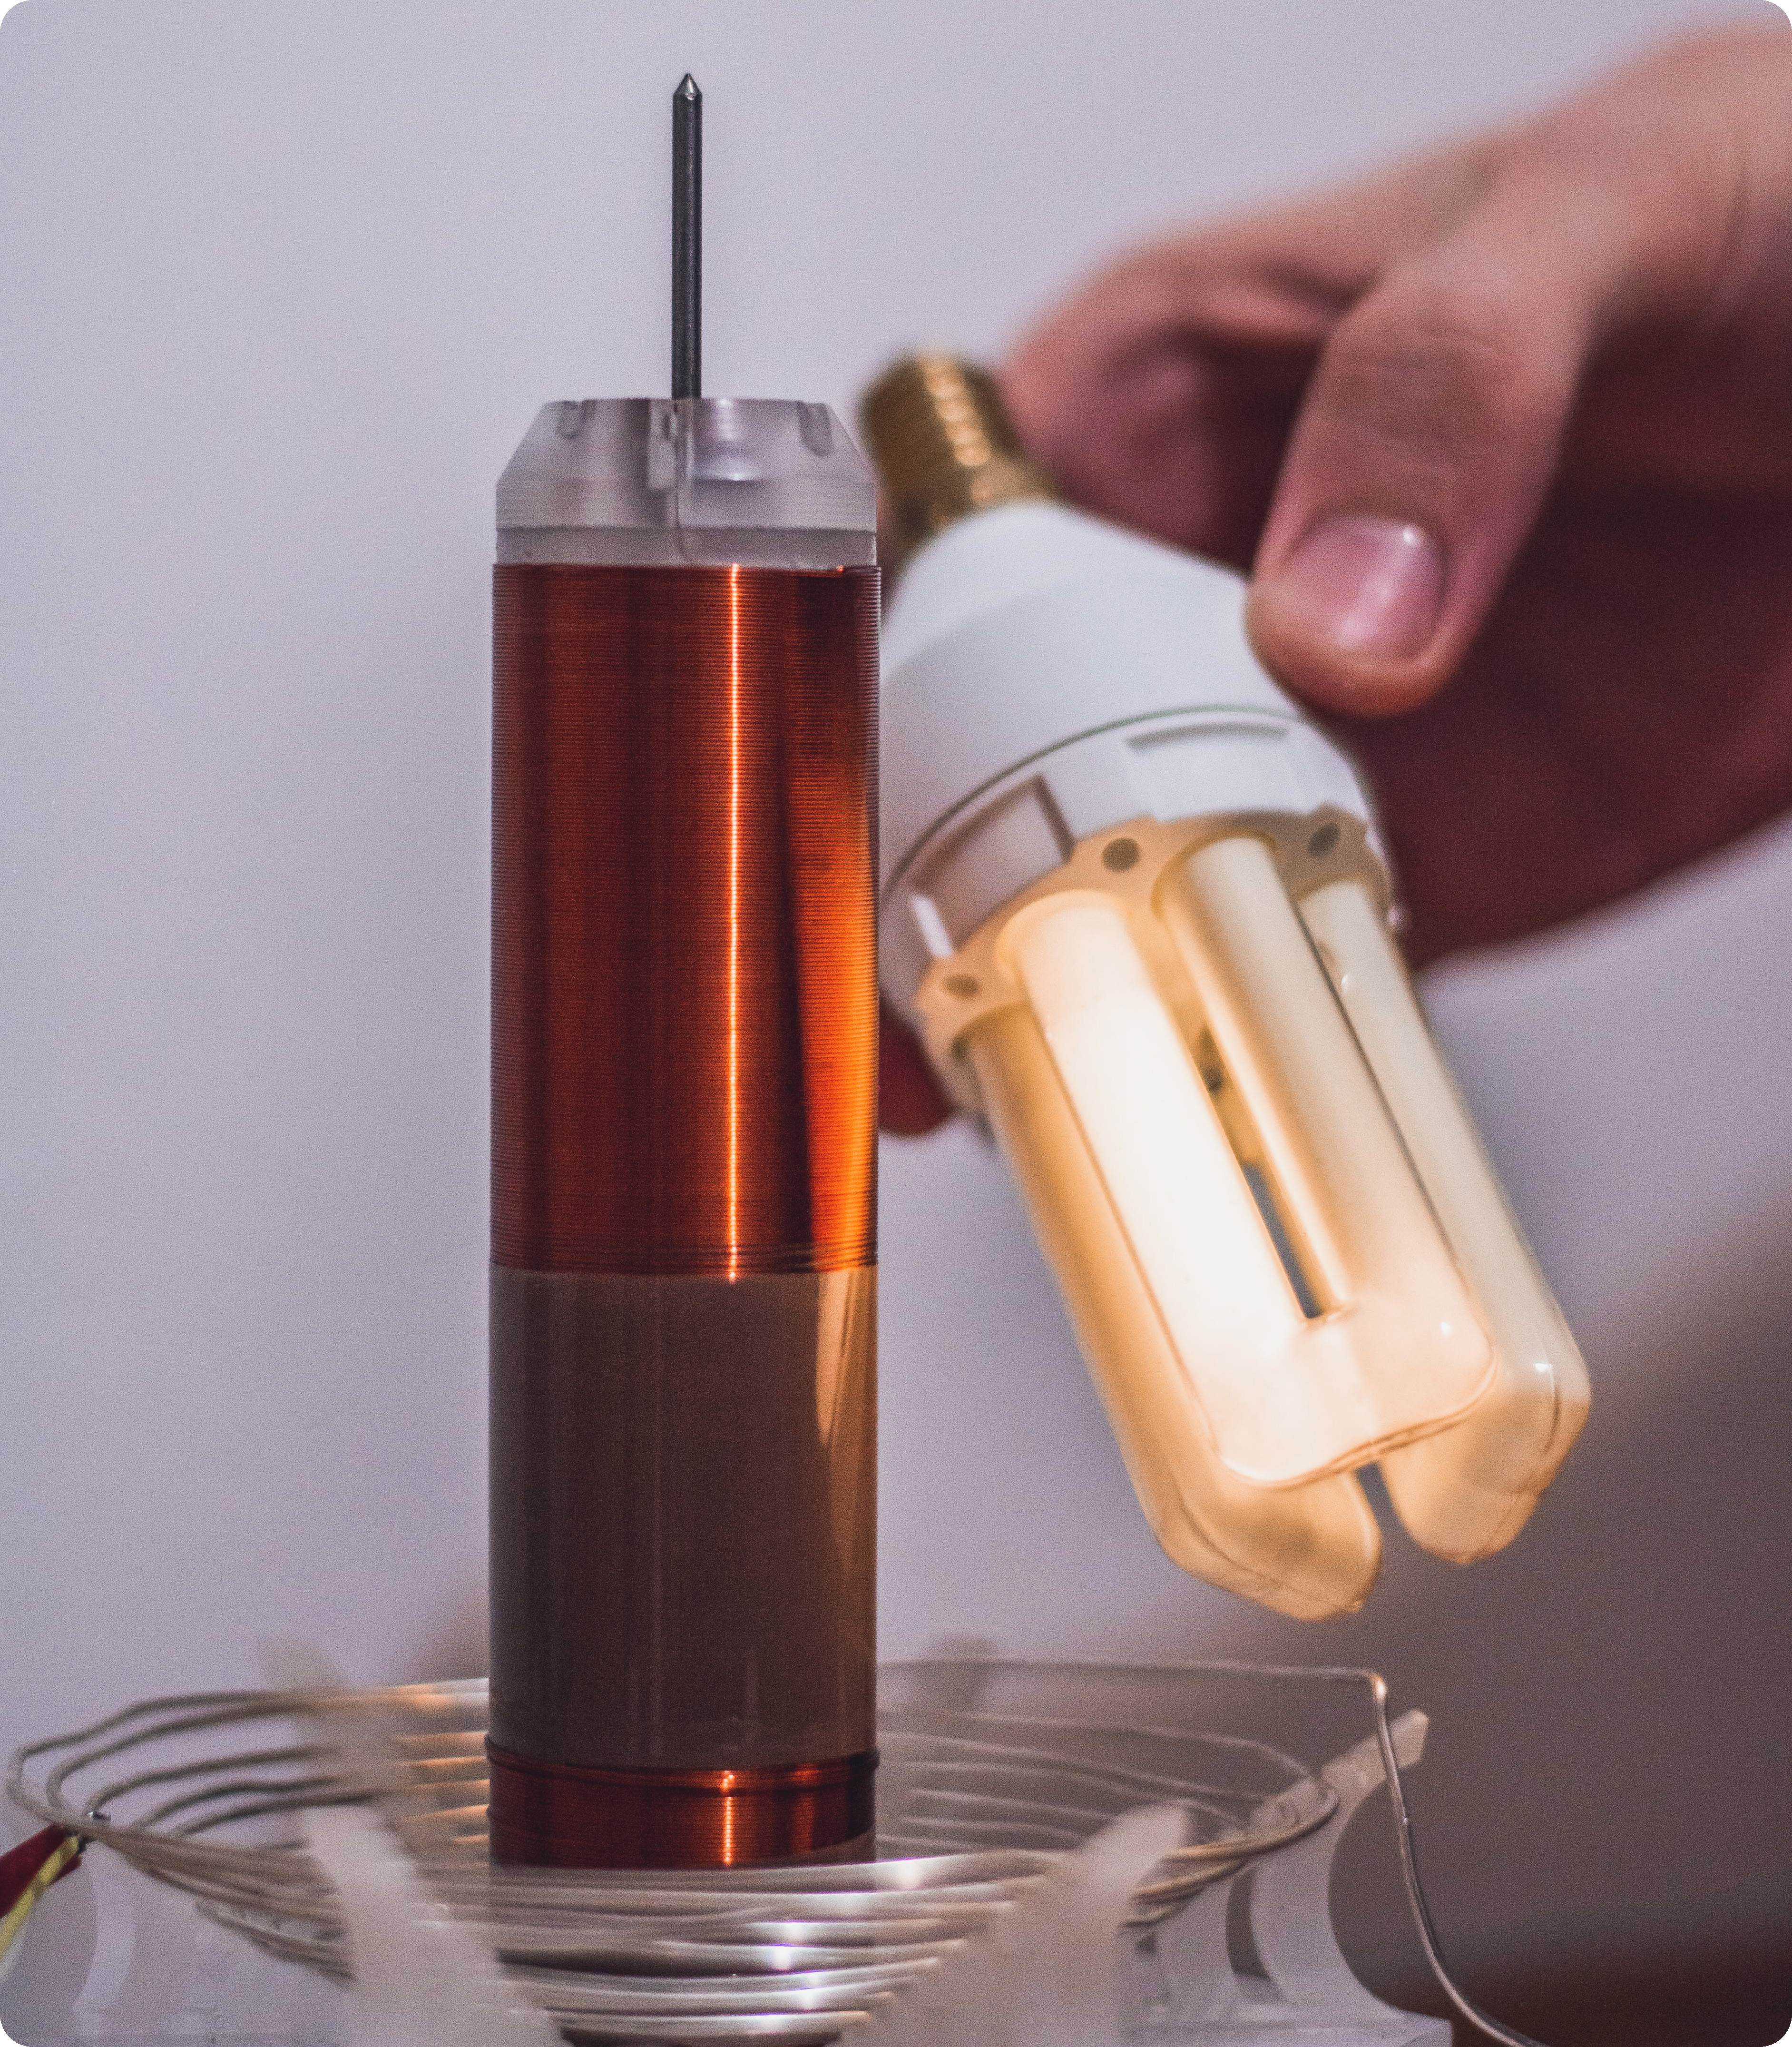
\includegraphics[width=0.7\textwidth]{simon/resources/blitzi2.jpg}
    \caption{Lighting a Lamp Wirelessly}
    \label{fig:lamp}
\end{figure}

% Todo
% 2.2   The Class-E Stage
% 3.x Practice
% 4.x Future Improvements

\pagelayout{wide} % No margins
\addpart{Design and Building}
\pagelayout{margin} % Restore margins
\setchapterstyle{kao}
\setchapterpreamble[u]{\margintoc}

\setcounter{chapter}{9}

\chapter{Casing}
\labch{ks-section-1}

AAAAA AAAAA AAAAA AAAAA AAAAA AAAAA AAAAA AAAAA AAAAA AAAAA AAAAA AAAAA AAAAA AAAAA AAAAA AAAAA AAAAA AAAAA AAAAA AAAAA AAAAA AAAAA AAAAA AAAAA AAAAA AAAAA AAAAA AAAAA AAAAA AAAAA AAAAA AAAAA AAAAA AAAAA AAAAA AAAAA AAAAA AAAAA AAAAA AAAAA AAAAA AAAAA AAAAA AAAAA AAAAA AAAAA AAAAA AAAAA AAAAA AAAAA AAAAA AAAAA AAAAA AAAAA AAAAA AAAAA AAAAA AAAAA AAAAA AAAAA AAAAA AAAAA AAAAA AAAAA AAAAA

\sidenote{Printed Circuit Board}
\todo[backgroundcolor=blue,
bordercolor=green!60!white, textcolor=red]{PDF Coil Construction aka Simons Buch auf Telegram}

\section{Envision}

AAAAA AAAAA AAAAA AAAAA AAAAA AAAAA AAAAA AAAAA AAAAA AAAAA AAAAA AAAAA AAAAA AAAAA AAAAA AAAAA AAAAA AAAAA AAAAA AAAAA AAAAA AAAAA AAAAA AAAAA AAAAA AAAAA AAAAA AAAAA AAAAA AAAAA AAAAA AAAAA AAAAA AAAAA AAAAA AAAAA AAAAA AAAAA AAAAA AAAAA AAAAA AAAAA AAAAA AAAAA AAAAA AAAAA AAAAA AAAAA AAAAA AAAAA AAAAA AAAAA AAAAA AAAAA AAAAA AAAAA AAAAA AAAAA AAAAA AAAAA AAAAA AAAAA AAAAA AAAAA AAAAA
\todo[backgroundcolor=blue,
bordercolor=green!60!white, textcolor=red]{Grob Design vorlage mit bild(in Inventor) aber nicht wie wir es umsetzen(aka die steher). Alles Modular sein tun}

\section{Materials}

AAAAA AAAAA AAAAA AAAAA AAAAA AAAAA AAAAA AAAAA AAAAA AAAAA AAAAA AAAAA AAAAA AAAAA AAAAA AAAAA AAAAA AAAAA AAAAA AAAAA AAAAA AAAAA AAAAA AAAAA AAAAA AAAAA AAAAA AAAAA AAAAA AAAAA AAAAA AAAAA AAAAA AAAAA AAAAA AAAAA AAAAA AAAAA AAAAA AAAAA AAAAA AAAAA AAAAA AAAAA AAAAA AAAAA AAAAA AAAAA AAAAA AAAAA AAAAA AAAAA AAAAA AAAAA AAAAA AAAAA AAAAA AAAAA AAAAA AAAAA AAAAA AAAAA AAAAA AAAAA AAAAA
\todo[backgroundcolor=blue,
bordercolor=green!60!white, textcolor=red]{Welche veraussetzung die materialen haben müssen und warum gewisse nicht in frage kommen. Berechnungen auch}

\section{Structure for the Coils}

AAAAA AAAAA AAAAA AAAAA AAAAA AAAAA AAAAA AAAAA AAAAA AAAAA AAAAA AAAAA AAAAA AAAAA AAAAA AAAAA AAAAA AAAAA AAAAA AAAAA AAAAA AAAAA AAAAA AAAAA AAAAA AAAAA AAAAA AAAAA AAAAA AAAAA AAAAA AAAAA AAAAA AAAAA AAAAA AAAAA 
\todo[backgroundcolor=blue,
bordercolor=green!60!white, textcolor=red]{Das Gerüst für die zwei spulen. Steher Desgin und funktion. Spitze mit Kupfer mit Spindel. Vlt erstes design mit Löt}

\section{It's not a Bug, it's a feature}

AAAAA AAAAA AAAAA AAAAA AAAAA AAAAA AAAAA AAAAA AAAAA AAAAA AAAAA AAAAA AAAAA AAAAA AAAAA AAAAA AAAAA AAAAA AAAAA AAAAA AAAAA AAAAA AAAAA AAAAA AAAAA AAAAA AAAAA AAAAA AAAAA AAAAA AAAAA AAAAA AAAAA AAAAA AAAAA AAAAA 
\todo[backgroundcolor=blue,
bordercolor=green!60!white, textcolor=red]{der Bug mit der Spitze aka Dach hohenverstellbar und wie. Auch Tests mit verschiedenen Anzahl an Kanten. Und aus was für einen Material, isolierung und so weita}

\section{Board Casing}

AAAAA AAAAA AAAAA AAAAA AAAAA AAAAA AAAAA AAAAA AAAAA AAAAA AAAAA AAAAA AAAAA AAAAA AAAAA AAAAA AAAAA AAAAA AAAAA AAAAA AAAAA AAAAA AAAAA AAAAA AAAAA AAAAA AAAAA AAAAA AAAAA AAAAA AAAAA AAAAA AAAAA AAAAA AAAAA AAAAA 
\todo[backgroundcolor=blue,
bordercolor=green!60!white, textcolor=red]{warum hexgon?}

\section{Final}

AAAAA AAAAA AAAAA AAAAA AAAAA AAAAA AAAAA AAAAA AAAAA AAAAA AAAAA AAAAA AAAAA AAAAA AAAAA AAAAA AAAAA AAAAA AAAAA AAAAA AAAAA AAAAA AAAAA AAAAA AAAAA AAAAA AAAAA AAAAA AAAAA AAAAA AAAAA AAAAA AAAAA AAAAA AAAAA AAAAA 
\todo[backgroundcolor=blue,
bordercolor=green!60!white, textcolor=red]{vlt was Ozonen machen wie zB desinfezieren}

\chapter{Printed Circuit Board}

\section{Why no Breadboards and Solutions}

AAAAA AAAAA AAAAA AAAAA AAAAA AAAAA AAAAA AAAAA AAAAA AAAAA AAAAA AAAAA AAAAA AAAAA AAAAA AAAAA AAAAA AAAAA AAAAA AAAAA AAAAA AAAAA AAAAA AAAAA AAAAA AAAAA AAAAA AAAAA AAAAA AAAAA AAAAA AAAAA AAAAA AAAAA AAAAA AAAAA 
\todo[backgroundcolor=blue,
bordercolor=green!60!white, textcolor=red]{der fakt das es bei dem hohen frequenzbereich und den kleinen capazitäten(datenblätter für breadboards). Unsere mit einzelnen Bauteilen bestückte Platinen}

\section{Essential Components}

AAAAA AAAAA AAAAA AAAAA AAAAA AAAAA AAAAA AAAAA AAAAA AAAAA AAAAA AAAAA AAAAA AAAAA AAAAA AAAAA AAAAA AAAAA AAAAA AAAAA AAAAA AAAAA AAAAA AAAAA AAAAA AAAAA AAAAA AAAAA AAAAA AAAAA AAAAA AAAAA AAAAA AAAAA AAAAA AAAAA 
\todo[backgroundcolor=blue,
bordercolor=green!60!white, textcolor=red]{geht in der simulierung aba nicht in da parxis. Design choices bei selbst erstellten bauteile. Massefläche warum und Desgin fehler bei Gehäuse bauteilen wie bei Spule und capazitator}

\section{Structure for the Coils}

AAAAA AAAAA AAAAA AAAAA AAAAA AAAAA AAAAA AAAAA AAAAA AAAAA AAAAA AAAAA AAAAA AAAAA AAAAA AAAAA AAAAA AAAAA AAAAA AAAAA AAAAA AAAAA AAAAA AAAAA AAAAA AAAAA AAAAA AAAAA AAAAA AAAAA AAAAA AAAAA AAAAA AAAAA AAAAA AAAAA 

\chapter{Future Ideas and Optimizations}



\pagelayout{wide} % No margins
\addpart{MIDI Interrupter}
\pagelayout{margin} % Restore margins
\setchapterstyle{kao}
\setchapterpreamble[u]{\margintoc}

\setcounter{chapter}{19}

\chapter{The MIDI Protocol}
\labch{mi-midi-protocol}


\section{Why use MIDI}

AAAAA AAAAA AAAAA AAAAA AAAAA AAAAA AAAAA AAAAA AAAAA AAAAA AAAAA AAAAA AAAAA AAAAA AAAAA AAAAA AAAAA AAAAA AAAAA AAAAA AAAAA AAAAA AAAAA AAAAA AAAAA AAAAA AAAAA AAAAA AAAAA AAAAA AAAAA AAAAA AAAAA AAAAA AAAAA AAAAA AAAAA AAAAA AAAAA AAAAA AAAAA AAAAA AAAAA AAAAA AAAAA AAAAA AAAAA AAAAA AAAAA AAAAA AAAAA AAAAA AAAAA AAAAA AAAAA AAAAA AAAAA AAAAA AAAAA AAAAA AAAAA AAAAA AAAAA AAAAA AAAAA

\section{Live MIDI ver MIDI Dateien}

AAAAA AAAAA AAAAA AAAAA AAAAA AAAAA AAAAA AAAAA AAAAA AAAAA AAAAA AAAAA AAAAA AAAAA AAAAA AAAAA AAAAA AAAAA AAAAA AAAAA AAAAA AAAAA AAAAA AAAAA AAAAA AAAAA AAAAA AAAAA AAAAA AAAAA AAAAA AAAAA AAAAA AAAAA AAAAA AAAAA AAAAA AAAAA AAAAA AAAAA AAAAA AAAAA AAAAA AAAAA AAAAA AAAAA AAAAA AAAAA AAAAA AAAAA AAAAA AAAAA AAAAA AAAAA AAAAA AAAAA AAAAA AAAAA AAAAA AAAAA AAAAA AAAAA AAAAA AAAAA AAAAA

\section{What is MIDI}

\subsection{General information about MIDI}

Musical Instrument Digital Interface short MIDI is a "Protocol" for exchanging musical Control program information between

\chapter{Programming the Interrupter}

\section{Choice of Hardware}

\appendix % From here onwards, chapters are numbered with letters, as is the appendix convention

\pagelayout{wide} % No margins
\addpart{Appendix}
\pagelayout{margin} % Restore margins

\input{chapters/appendix.tex}

%----------------------------------------------------------------------------------------

\backmatter % Denotes the end of the main document content
\setchapterstyle{plain} % Output plain chapters from this point onwards

%----------------------------------------------------------------------------------------
%	BIBLIOGRAPHY
%----------------------------------------------------------------------------------------

% The bibliography needs to be compiled with biber using your LaTeX editor, or on the command line with 'biber main' from the template directory

\defbibnote{bibnote}{Here are the references in citation order.\par\bigskip} % Prepend this text to the bibliography
\printbibliography[heading=bibintoc, title=Bibliography, prenote=bibnote] % Add the bibliography heading to the ToC, set the title of the bibliography and output the bibliography note

%----------------------------------------------------------------------------------------
%	NOMENCLATURE
%----------------------------------------------------------------------------------------

% The nomenclature needs to be compiled on the command line with 'makeindex main.nlo -s nomencl.ist -o main.nls' from the template directory

\nomenclature{SSTC}{Solid State Tesla Coil}
\nomenclature{CW}{Continuous wave}

\renewcommand{\nomname}{Notation} % Rename the default 'Nomenclature'
\renewcommand{\nompreamble}{The next list describes several symbols that will be later used within the body of the document.} % Prepend this text to the nomenclature

\printnomenclature % Output the nomenclature

%----------------------------------------------------------------------------------------
%	GLOSSARY
%----------------------------------------------------------------------------------------

% The glossary needs to be compiled on the command line with 'makeglossaries main' from the template directory

\newglossaryentry{computer}{
	name=computer,
	description={is a programmable machine that receives input, stores and manipulates data, and provides output in a useful format}
}

% Glossary entries (used in text with e.g. \acrfull{fpsLabel} or \acrshort{fpsLabel})
\newacronym[longplural={Frames per Second}]{fpsLabel}{FPS}{Frame per Second}
\newacronym[longplural={Tables of Contents}]{tocLabel}{TOC}{Table of Contents}

\setglossarystyle{listgroup} % Set the style of the glossary (see https://en.wikibooks.org/wiki/LaTeX/Glossary for a reference)
\printglossary[title=Special Terms, toctitle=List of Terms] % Output the glossary, 'title' is the chapter heading for the glossary, toctitle is the table of contents heading

%----------------------------------------------------------------------------------------
%	INDEX
%----------------------------------------------------------------------------------------

% The index needs to be compiled on the command line with 'makeindex main' from the template directory

\printindex % Output the index

%----------------------------------------------------------------------------------------
%	BACK COVER
%----------------------------------------------------------------------------------------

% If you have a PDF/image file that you want to use as a back cover, uncomment the following lines

%\clearpage
%\thispagestyle{empty}
%\null%
%\clearpage
%\includepdf{cover-back.pdf}

%----------------------------------------------------------------------------------------

\end{document}
